\documentclass[20pt]{article}
% remarkable size: 1404×1872 pixels
% 14.625 X  19.5
\usepackage[paperwidth=1404px,paperheight=1872px,top=0.5in,bottom=0.5in,left=0.5in,right=0.5in]{geometry}
\usepackage{calc}
\usepackage{tikz}
\thispagestyle{empty}
\newlength{\wholeboxwd}
    \setlength{\wholeboxwd}{0.99\textwidth}
\newlength{\wholeboxht}
    \setlength{\wholeboxht}{0.99\textheight}
%
\newlength{\cuewd}
    \setlength{\cuewd}{0.3\wholeboxwd}
\newlength{\summht}
    \setlength{\summht}{0.15\wholeboxht}
\newlength{\cgridht}
    \setlength{\cgridht}{\wholeboxht-\summht}
\newlength{\cgridwd}
    \setlength{\cgridwd}{\wholeboxwd-\cuewd}
\newlength{\xorig}
\newlength{\yorig}
\setlength{\xorig}{0cm}
\setlength{\yorig}{0cm}

\begin{document}

\begin{center}
\begin{tikzpicture}

% put lines in the large right "notes" section

\foreach \i in {0,60,...,1450}{
  \draw[lightgray] (\cuewd,\summht +\i) -- (\wholeboxwd,\summht +\i) ;
}

% ($(current page.north west)+(0,-\i)$) -- ($(current page.north east)+(0,-\i)$);



%% big graph paper
%\draw[step=.5cm,gray!80,thin] (\cuewd,\summht) grid (\wholeboxwd,\wholeboxht) ;
%% Optional: -- small graph paper
%\draw[step=.25cm,gray!30,thin] (\cuewd,\summht) grid (\wholeboxwd,\wholeboxht);
% Summary, top:
\draw [line width=.2pt] (\xorig,\summht) -- (\wholeboxwd,\summht);
% Grid, left:
\draw [line width=.2pt] (\cuewd,\summht) -- (\cuewd,\wholeboxht);
% Draw the big box:
\draw (\xorig,\yorig) rectangle (\wholeboxwd,\wholeboxht);

% put lines in the bottom "to do" section.
\foreach \i in {0,50,...,200}{
\draw(\xorig,\yorig+\i) -- (\wholeboxwd / 2.05, \yorig+\i);
\draw(\wholeboxwd-\wholeboxwd/2.05 ,\yorig+\i) -- (\wholeboxwd , \yorig+\i);

}
\node[anchor=west] at (0.25,\wholeboxht-2em) {\textbf{\Huge Details/Notes:}};
\node[anchor=west] at (0.25,\summht-2em){\textbf{\Huge To Do:}};


\node[anchor=west,fill=white] at (\cuewd+0em,\wholeboxht-2em) {\textbf{\Huge\ Notes:\ }};
%% \node[anchor=west] at (0.25,\wholeboxht+2em){%
%%     \parbox[t]{\cuewd}{Subject:\par\smallskip Date:}%
%% };
\end{tikzpicture}
\end{center}

\end{document}
